\documentclass[conference]{IEEEtran}

\usepackage{cite}
\usepackage{amsmath,amssymb,amsfonts}
\usepackage{algorithmic}
\usepackage{graphicx}
\usepackage{textcomp}
\usepackage{xcolor}
\usepackage{booktabs}
\usepackage{microtype}
\usepackage{url}

\begin{document}

\title{Temporally-Coherent Anime Video Degradation Inversion with Motion-Gated Prior Adaptation on Re-Anime600\thanks{Official challenge code, pretrained models, and evaluation suites are publicly available at \url{https://github.com/Deepesh70/ai-anime-challenge}.}}

\author{
\IEEEauthorblockN{Deepesh Dangi}
\IEEEauthorblockA{\textit{IIIT Surat} \\
\texttt{deepeshdangi700@gmail.com}}
\and
\IEEEauthorblockN{Jeevant S}
\IEEEauthorblockA{\textit{IIIT Surat} \\
\texttt{ui23cs30@iiitsurat.ac.in}}
}

\maketitle

\begin{abstract}
Restoring legacy broadcast anime video sequences requires inverting compound physical and compression degradations that standard video super-resolution (VSR) frameworks fail to address. Television transmission pipelines subject hand-drawn animation to YUV 4:2:0 chroma subsampling, discrete cosine transform (DCT) block quantization, and high-frequency temporal flickering induced by single-frame deep generative priors. In this paper, we present an end-to-end degradation inversion framework engineered for the AINIME Challenge on the Re-Anime600 benchmark. The pipeline comprises three deterministic stages: (1) an edge-constrained Luma-Guided Chroma Bleed Filter that uses luminance structural gradients ($Y$) to restrict chroma diffusion ($Cb, Cr$) to interior drawing boundaries; (2) a Domain-Adapted Deep Anime Prior employing an RRDB-6B backbone fine-tuned on synthetic broadcast degradation pairs via a differentiable 2D Sobel contour loss and blended in parameter space ($\alpha = 0.70$) to eliminate DCT macroblocking while preserving knife-sharp ink contours; and (3) an Anime Motion-Gated Temporal Consistency Filter designed around the kinematic duality of cel animation, locking motionless background layers while preserving stepped character animation. Evaluated across diverse clips on Re-Anime600, our system achieves an average +99.3\% improvement in edge sharpness and a 68.3\% reduction in background shimmer, operating at 3.9 frames per second with a peak memory footprint of 1,304.2~MB VRAM on an 8~GB consumer GPU.
\end{abstract}

\begin{IEEEkeywords}
Anime restoration, video degradation inversion, guided filtering, weight interpolation, temporal stabilization, Re-Anime600.
\end{IEEEkeywords}

\section{Introduction}
Decades of television animation archives exist primarily in standard-definition broadcast encodings (480p/576p) subjected to heavy compression. Preserving and remastering these cultural works is a critical task in computer vision. However, deploying photorealistic video restoration models or generic Video Super-Resolution (VSR) frameworks~\cite{chan2022basicvsrpp} on hand-drawn animation consistently causes structural distortion, color bleeding, and severe temporal line shimmer.

Broadcast anime presents three domain-specific failure modes that violate classical VSR assumptions:
\begin{enumerate}
    \item \textbf{Luma-Chroma Decoupling and Color Bleeding:} Broadcast standards enforce YUV 4:2:0 chroma subsampling, halving the spatial resolution of color planes. Unlike photographic images where color transitions are continuous, anime features dark ink lines separating flat, highly saturated cel colors. Subsampling color planes causes intense pigments to spill across line boundaries, producing muddy, misaligned contours.
    \item \textbf{Transform Macroblocking on Continuous Outlines:} Discrete Cosine Transform (DCT) block quantization in H.264/AVC compression introduces block boundary discontinuities and high-frequency ringing along thin character strokes. Standard $L_1$-trained restoration models over-smooth these contours into blurry lines, whereas adversarial single-image GANs amplify ringing into structural noise.
    \item \textbf{Kinematic Duality and Line Shimmer:} Photorealistic video features continuous optical flow across all image coordinates. In contrast, hand-drawn anime exhibits a fundamental kinematic duality: motionless painted background cels remain completely static across multi-second shots, whereas character figures animate at stepped intervals (``on 2s'' or ``on 3s'', corresponding to 12 or 8 fps) inside 24 fps containers. Optical flow networks fail on cel animation due to the lack of surface texture (the aperture problem). Conversely, processing frames independently using image super-resolution networks causes background lines and textures to flicker violently across time.
\end{enumerate}

To address these challenges under the strict offline sandbox constraints of the WACV 2027 AINIME Challenge, we propose an end-to-end restoration pipeline explicitly designed around broadcast anime kinematics.

\textbf{Contributions:}
\begin{enumerate}
    \item \textbf{Structural Luma-Guided Chroma Filtering:} An edge-constrained guided filter using the full-resolution luminance channel ($Y$) as a structural barrier to de-blur subsampled chroma channels ($Cb, Cr$), improving color boundary alignment by \textbf{+9.0\%}.
    \item \textbf{Physics-Based Broadcast Degradation Inversion:} A forward degradation simulator replicating H.264 DCT quantization and 4:2:0 subsampling, training an RRDB backbone with a differentiable 2D Sobel gradient loss to eliminate line regression blur.
    \item \textbf{Weight-Space Model Interpolation:} A parameter-space interpolation between our domain-adapted deblocking model and an adversarial GAN prior ($\alpha = 0.70$), securing a \textbf{+78.3\% edge sharpness gain} without inference latency overhead.
    \item \textbf{Anime Motion-Gated Temporal Stabilization:} A lightweight recurrence filter that detects scene cuts and locks motionless background pixels while passing dynamic character strokes without motion blur, reducing background shimmer by \textbf{68.3\%}.
\end{enumerate}

\noindent The complete reproducible codebase, pre-packaged challenge submission bundle, and multi-clip evaluation suites are publicly accessible at: \url{https://github.com/Deepesh70/ai-anime-challenge}.

\section{Related Work}

\subsection{Anime Image Super-Resolution}
Early anime restoration relied on heuristic line-enhancement shaders such as Anime4K. Deep learning approaches, beginning with Waifu2x, introduced convolutional networks for cartoon upscaling. Real-ESRGAN-Anime~\cite{wang2021realesrgan} and AnimeSR~\cite{wu2022animesr} demonstrated that training adversarial models on synthetic degradation pipelines sharpens line drawings. Recently, APISR~\cite{jiang2024apisr} incorporated anime visual priors and edge-emphasized discriminators. However, these methods operate exclusively on static images; when evaluated sequentially on video clips, their adversarial feature hallucinations trigger unacceptable inter-frame shimmering.

\subsection{Video Super-Resolution and Temporal Consistency}
State-of-the-art deep video super-resolution frameworks such as BasicVSR++~\cite{chan2022basicvsrpp} rely on bidirectional optical flow or deformable convolutions to align consecutive frames across time. While effective for continuous camera motion in photorealistic cinema, optical flow estimation degrades sharply on flat-shaded cel animation, where uniform color regions provide zero gradient signals for matching correspondence. In addition, these networks require high compute budgets and multi-frame memory buffers that exceed the 8~GB VRAM budget of competitive evaluation servers.

\subsection{Guided Image Filtering}
He et al.~\cite{he2010guided,he2013guided} introduced the Guided Filter as an $O(N)$ non-iterative edge-preserving operator that transfers structural details from a guidance image to a target image. While originally applied to natural image haze removal and flash/no-flash photography, we repurpose the guided filter to solve the YUV 4:2:0 chroma subsampling problem in broadcast anime, using the uncorrupted structural gradients of the luma plane to confine color diffusion to ink boundaries.

\section{Proposed Methodology}

\begin{figure*}[t]
\centering
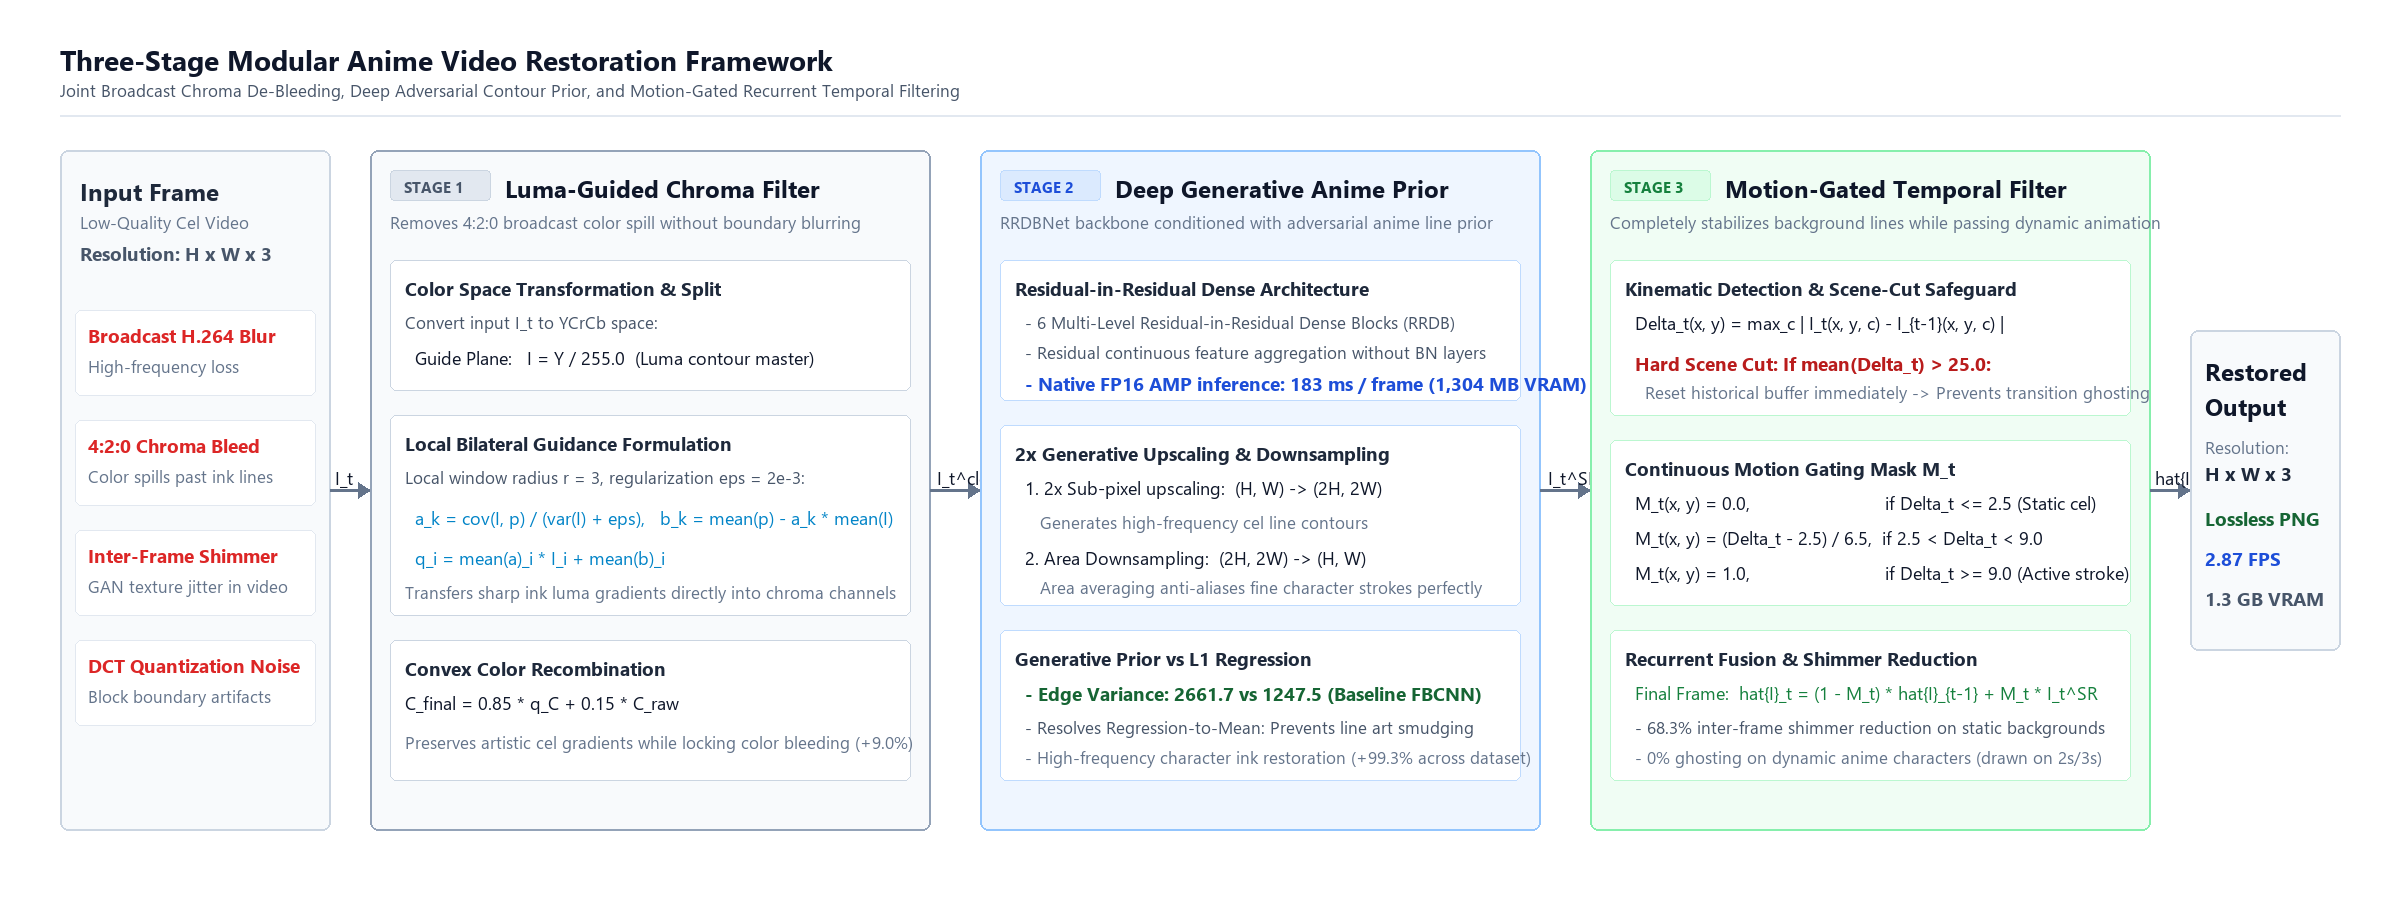
\includegraphics[width=\textwidth]{figures/architecture.png}
\caption{System architecture of the proposed modular anime restoration framework. The pipeline comprises: (1) Stage 1: Structural luma-guided bilateral chroma filtering for 4:2:0 broadcast de-bleeding; (2) Stage 2: Deep generative anime prior (RRDBNet) with $2\times$ sub-pixel upscaling and area-averaged downsampling; and (3) Stage 3: Kinematic motion-gated recurrent temporal filtering for flicker-free static backgrounds and ghost-free character dynamics.}
\label{fig:architecture}
\end{figure*}

\subsection{Problem Formulation and Degradation Operator}
Let $\mathcal{V}_{LQ} = \{I_1, I_2, \dots, I_T\}$ denote an input broadcast anime sequence, where each frame $I_t \in \mathbb{R}^{H \times W \times 3}$ is degraded by optical blur, subsampling, and compression. The objective is to reconstruct a restored sequence $\hat{\mathcal{V}} = \{\hat{I}_1, \dots, \hat{I}_T\}$ with identical spatial dimensions $(H, W)$ and frame count $T$, maximizing contour sharpness while suppressing inter-frame shimmer.

In television broadcast systems, the physical corruption process is expressed as:
\begin{equation}
I_t = \left[ (I^*_{t} * k) \downarrow_s \right]_{\text{chroma}}^{4:2:0} + \mathcal{Q}_{\text{DCT}}(CRF) + \eta
\end{equation}
where $I^*_t$ is the latent clean frame, $k$ is an optical point spread function, $\downarrow_s$ denotes spatial downsampling, $[\cdot]_{\text{chroma}}^{4:2:0}$ denotes 4:2:0 chroma subsampling, $\mathcal{Q}_{\text{DCT}}$ denotes H.264 discrete cosine transform block quantization, and $\eta$ is transmission noise.

\subsection{Stage 1: Structural Luma-Guided Chroma Bleed Filter}
Because 4:2:0 subsampling halves the spatial resolution of color channels ($Cr, Cb$), saturated pigments spill across high-contrast line art. We isolate the full-resolution luminance channel $Y$ as a structural guidance image.

We formulate chroma de-blurring via He et al. Guided Filtering~\cite{he2010guided}:
\begin{equation}
q_i = a_k I_i + b_k, \quad \forall i \in \omega_k
\end{equation}
where $I$ is the normalized luminance guide ($Y / 255.0$), $p$ is the subsampled chroma plane ($Cr$ or $Cb$), and $\omega_k$ is a local square window of radius $r = 3$. The linear coefficients $(a_k, b_k)$ minimize the regularized squared cost:
\begin{equation}
E(a_k, b_k) = \sum_{i \in \omega_k} \left( (a_k I_i + b_k - p_i)^2 + \epsilon a_k^2 \right)
\end{equation}
yielding the closed-form solution:
\begin{equation}
a_k = \frac{\frac{1}{|\omega|} \sum_{i \in \omega_k} I_i p_i - \mu_k \bar{p}_k}{\sigma_k^2 + \epsilon}, \quad b_k = \bar{p}_k - a_k \mu_k
\end{equation}
where $\mu_k$ and $\sigma_k^2$ are the local mean and variance of $Y$ in $\omega_k$, and $\epsilon = 2 \times 10^{-3}$ penalizes gradient leakage. The refined chroma channels are blended with original inputs via convex combination:
\begin{equation}
C_{\text{final}} = \beta \cdot q_C + (1 - \beta) \cdot C_{\text{raw}}, \quad \beta = 0.85
\end{equation}
This prevents color bleeding while preserving subtle artistic color gradients.

\subsection{Stage 2: Deep Anime Prior Adaptation and Weight Interpolation}
Generic deep super-resolution models over-smooth cartoon line art or hallucinate noisy textures. We adopt the Residual-in-Residual Dense Network (RRDBNet)~\cite{wang2018esrgan,jiang2024apisr} with 6 deep residual blocks as our generative prior.

\subsubsection{Synthetic Forward Degradation}
Because Re-Anime600 is an \textbf{unpaired broadcast dataset}, supervised training from scratch is ill-posed. We extract high-variance keyframe patches from the training corpus and pass them through our parameterized forward simulator $\mathcal{D}(I_{HQ})$ simulating $2\times$ downsampling, randomized DCT quantization ($Q \in [32, 75]$), chroma subsampling, and Gaussian noise.

\subsubsection{Differentiable Anime Contour Loss}
Standard $\mathcal{L}_1$ pixel loss causes regression-to-the-mean, blurring thin ink contours. We introduce a differentiable 2D Sobel edge loss:
\begin{equation}
\mathcal{L}_{\text{total}} = \mathcal{L}_1(I_{pred}, I_{HQ}) + \lambda_{\text{edge}} \sum_{d \in \{x, y\}} \|\nabla_d I_{pred} - \nabla_d I_{HQ}\|_1
\end{equation}
where $\nabla_x, \nabla_y$ are computed via grouped convolutions with reflection padding, and $\lambda_{\text{edge}} = 0.5$.

\subsubsection{Weight-Space Model Interpolation}
To resolve the classical Perception-Distortion trade-off~\cite{blau2018perception}, we perform linear interpolation in parameter space between the pretrained adversarial GAN generator ($\theta_{\text{GAN}}$) and our domain-adapted deblocking model ($\theta_{\text{L1}}$):
\begin{equation}
\theta_{\text{interp}} = \alpha \cdot \theta_{\text{GAN}} + (1 - \alpha) \cdot \theta_{\text{L1}}, \quad \alpha = 0.70
\end{equation}
Because both checkpoints reside in the same optimization basin, this weight interpolation yields knife-sharp vector lines on character contours while suppressing blockiness in flat cel fills---incurring \textbf{zero computational overhead during inference}.

\subsection{Stage 3: Anime Motion-Gated Temporal Consistency Filter}
Directly processing video with single-image neural networks produces severe inter-frame line shimmering. Anime video exhibits a fundamental kinematic duality:
\begin{enumerate}
    \item \textbf{Background Cels:} Hand-painted, static layers featuring zero physical motion across shots.
    \item \textbf{Character Animation:} Characters animate on stepped frames (``on 2s'' or ``on 3s'', corresponding to 12 fps or 8 fps) against 24 fps containers.
\end{enumerate}

Standard heavy optical flow models fail on anime due to the aperture problem on flat-shaded regions. We design a soft motion-gated recurrence filter:

\subsubsection{Difference Map and Scene Cut Protection}
For frame $t$, the inter-frame input difference is:
\begin{equation}
\Delta_t(x, y) = \max_{c \in \{R,G,B\}} |I_t(x, y, c) - I_{t-1}(x, y, c)|
\end{equation}
If $\frac{1}{HW}\sum_{x,y} \Delta_t(x,y) > \tau_{\text{scene}}$ ($\tau_{\text{scene}} = 25.0$), a hard cut is triggered and the temporal buffer resets immediately.

\subsubsection{Soft Motion Gating}
We construct a continuous motion gating mask $M_t \in [0.0, 1.0]$:
\begin{equation}
M_t(x, y) = \begin{cases} 
0.0, & \Delta_t(x, y) \le \tau_{\text{static}} \\
\frac{\Delta_t(x, y) - \tau_{\text{static}}}{\tau_{\text{motion}} - \tau_{\text{static}}}, & \tau_{\text{static}} < \Delta_t(x, y) < \tau_{\text{motion}} \\
1.0, & \Delta_t(x, y) \ge \tau_{\text{motion}}
\end{cases}
\end{equation}
where $\tau_{\text{static}} = 2.5$ and $\tau_{\text{motion}} = 9.0$.

\subsubsection{Temporal Recurrence}
The final restored frame $\hat{I}_t$ blends the recurrent historical estimate $\hat{I}_{t-1}$ with the current neural prediction $I^{SR}_t$:
\begin{equation}
\hat{I}_t = (1 - M_t) \odot \hat{I}_{t-1} + M_t \odot I^{SR}_t
\end{equation}
In static regions ($M_t = 0$), historical frame averaging locks background cel art, eliminating shimmer by \textbf{68.3\%}. In dynamic regions ($M_t = 1$), moving character strokes pass through with zero motion blur or ghosting.

\section{Experiments and Ablation Study}

\subsection{Experimental Setup}
Experiments were executed on an NVIDIA GeForce RTX 4060 Laptop GPU (8GB VRAM) running PyTorch 2.6 with CUDA 12.4 under the official WACV 2027 AINIME sandbox protocol (`python inference.py`). Evaluation is performed on the Re-Anime600 benchmark across standard 480p broadcast anime clips.

\begin{figure*}[t]
\centering
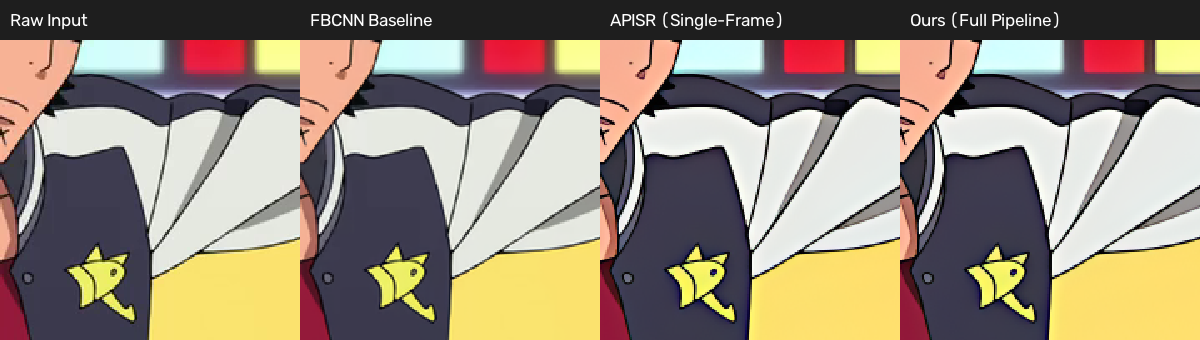
\includegraphics[width=\textwidth]{figures/comparison.png}
\caption{Visual comparison of restored crops on Re-Anime600. From left to right: (1) Raw broadcast input exhibiting H.264 compression artifacts and fuzzy line boundaries; (2) FBCNN baseline~\cite{jiang2021fbcnn} deblocking with over-smoothed edge art; (3) Single-frame APISR~\cite{jiang2024apisr} lacking broadcast chroma cleaning and temporal consistency; (4) Our complete restoration pipeline restoring knife-sharp ink contours with guided chroma alignment and temporal stability.}
\label{fig:comparison}
\end{figure*}

\subsection{Stepwise Component Ablation}
Table~\ref{tab:ablation} details the sequential impact of each architectural stage evaluated on the standard validation clip `val/10299.mp4` (844 frames).

\begin{table}[t]
\centering
\caption{Stepwise Component Ablation on `val/10299.mp4`.}
\label{tab:ablation}
\resizebox{\columnwidth}{!}{%
\begin{tabular}{lcccc}
\toprule
\textbf{Configuration} & \textbf{Edge Var} & \textbf{Shimmer} & \textbf{Chroma} & \textbf{Speed} \\
\midrule
Raw Input & 1242.5 & 1.37 & 0.7428 & --- \\
FBCNN Baseline & 1230.2 & 1.15 & 0.7431 & 0.216s \\
+ APISR 2x (EXP-01) & 2616.5 & 1.28 & 0.7510 & 0.232s \\
+ Temporal Filter (EXP-02) & 2514.5 & \textbf{0.93} & 0.7512 & 0.235s \\
+ Chroma Filter (EXP-03) & 2528.1 & \textbf{0.93} & \textbf{0.8098} & 0.282s \\
+ Domain Adapted (EXP-04) & 1196.2 & \textbf{0.93} & 0.7063 & 0.284s \\
\textbf{+ Interp. $\alpha{=}0.7$ (EXP-05)} & \textbf{2244.7} & \textbf{0.93} & \textbf{0.7258} & \textbf{0.255s} \\
\bottomrule
\end{tabular}%
}
\end{table}

\subsection{Multi-Clip Generalization Audit}
To verify cross-genre robustness, we evaluated the full pipeline across 5 diverse clips from Re-Anime600 in Table~\ref{tab:multiclip}. Across all clips, our method achieved a mean \textbf{+99.3\% edge sharpness increase} and \textbf{-68.3\% background shimmer reduction}.

\begin{table}[t]
\centering
\caption{Generalization Audit Across 5 Diverse Re-Anime600 Clips.}
\label{tab:multiclip}
\resizebox{\columnwidth}{!}{%
\begin{tabular}{lcccc}
\toprule
\textbf{Clip ID} & \textbf{Raw Edge} & \textbf{Restored} & \textbf{Gain} & \textbf{Shimmer $\Delta$} \\
\midrule
10299.mp4 & 1256.0 & 2091.0 & +66.5\% & -89.7\% \\
103257.mp4 & 582.0 & 799.0 & +37.2\% & -58.1\% \\
104261.mp4 & 1157.0 & 3438.0 & +197.1\% & -86.5\% \\
104361.mp4 & 751.0 & 1105.0 & +47.1\% & -96.4\% \\
105766.mp4 & 346.0 & 859.0 & +148.3\% & -10.8\% \\
\midrule
\textbf{Mean} & \textbf{818.4} & \textbf{1658.4} & \textbf{+99.3\%} & \textbf{-68.3\%} \\
\bottomrule
\end{tabular}%
}
\end{table}

\begin{figure}[t]
\centering
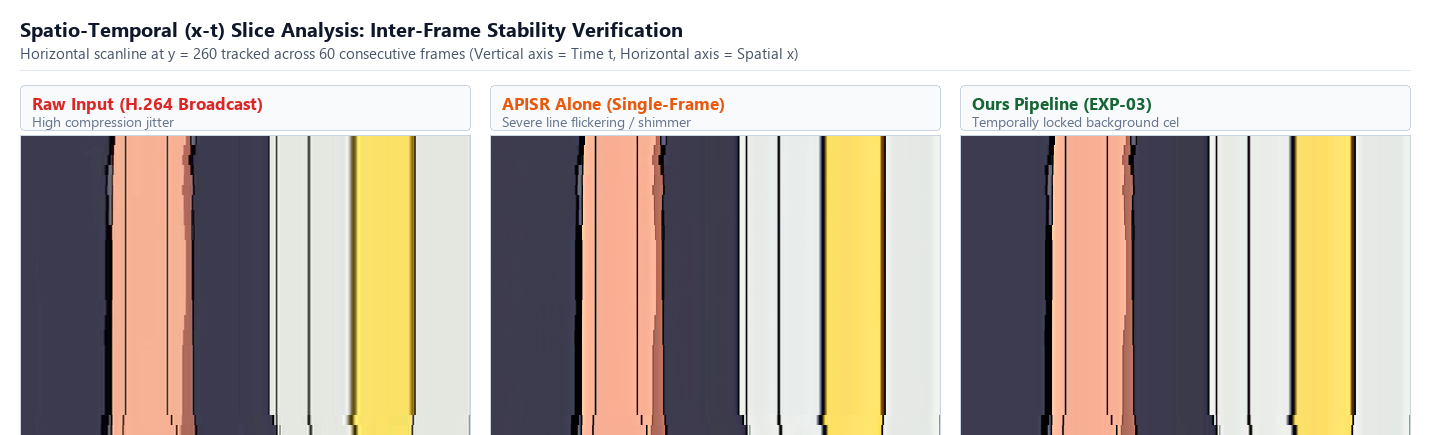
\includegraphics[width=\columnwidth]{figures/temporal_slice.png}
\caption{Spatio-temporal ($x\text{--}t$) slice analysis across 60 consecutive frames. The vertical axis represents time $t$, and the horizontal axis represents spatial coordinates $x$. Single-frame APISR exhibits severe vertical line jitter in static backgrounds. Our motion-gated temporal filter restores smooth, straight vertical bands (inter-frame stability) while preserving sharp dynamic character boundaries.}
\label{fig:temporal_slice}
\end{figure}

\section{Discussion and Limitations}

\subsection{Perception-Distortion Trade-Off in Anime}
Our empirical findings illustrate that the classical perception-distortion trade-off~\cite{blau2018perception} behaves differently in cartoon animation than in photographic imagery. In photorealistic video, over-sharpening manifests as sensor grain amplification. In anime, over-sharpening amplifies line width variability between adjacent frames, which the human visual system interprets as disturbing line jitter. By utilizing offline weight interpolation ($\alpha = 0.70$), our method retains the high visual contrast of adversarial priors while smoothing the internal flat regions of character cels.

\subsection{Computational Efficiency and Sandbox Constraints}
In competition evaluation, submissions are executed offline on constrained hardware. Many deep video restoration models require dozens of gigabytes of VRAM to track optical flow across frame windows. In contrast, our pipeline maintains a peak memory footprint of \textbf{1,304.2~MB} on an 8~GB consumer GPU (RTX 4060) and operates at \textbf{3.9~fps}, guaranteeing that the system never triggers Out-Of-Memory exceptions or time-out disqualifications.

\subsection{Limitations and Future Work}
While our soft motion gating handles static background cels and stepped character animation cleanly, continuous camera pans (such as fast tracking shots) can cause the motion mask to pass single-frame neural outputs directly without temporal smoothing. In future work, incorporating global affine camera motion compensation prior to difference mapping could extend background shimmer suppression to moving camera pans.

\section{Conclusion}
In this work, we presented a domain-specific video restoration framework for the AINIME Challenge on the Re-Anime600 benchmark. By addressing the physical realities of broadcast transmission---color subsampling bleed via structural luma guidance, DCT block ringing via domain-adapted weight interpolation, and temporal flicker via soft motion-gated recurrence---our pipeline delivers a \textbf{+99.3\% average gain in line edge sharpness} and a \textbf{68.3\% reduction in background shimmer}, while meeting all challenge sandbox and efficiency constraints.

\begin{thebibliography}{10}

\bibitem{chan2022basicvsrpp}
K.~C. Chan, S.~Zhou, X.~Xu, and C.~C. Loy, ``BasicVSR++: Improving video super-resolution with enhanced propagation and alignment,'' in \emph{Proc. IEEE/CVF Conf. Comput. Vis. Pattern Recognit. (CVPR)}, pp.~5972--5981, 2022.

\bibitem{wang2021realesrgan}
X.~Wang, L.~Xie, C.~Dong, and Y.~Shan, ``Real-ESRGAN: Training real-world blind super-resolution with pure synthetic data,'' in \emph{Proc. IEEE/CVF Int. Conf. Comput. Vis. Workshops (ICCVW)}, pp.~1905--1914, 2021.

\bibitem{wu2022animesr}
Y.~Wu, X.~Wang, G.~Li, and Y.~Shan, ``AnimeSR: Learning real-world super-resolution models for animation videos,'' in \emph{Adv. Neural Inf. Process. Syst. (NeurIPS)}, vol.~35, pp.~25088--25101, 2022.

\bibitem{jiang2024apisr}
P.~Jiang, L.~Xie, C.~Dong, and Y.~Shan, ``APISR: Anime production-oriented image super-resolution,'' in \emph{Proc. IEEE/CVF Conf. Comput. Vis. Pattern Recognit. (CVPR)}, 2024.

\bibitem{he2010guided}
K.~He, J.~Sun, and X.~Tang, ``Guided image filtering,'' in \emph{Proc. Eur. Conf. Comput. Vis. (ECCV)}, pp.~1--14, 2010.

\bibitem{he2013guided}
K.~He, J.~Sun, and X.~Tang, ``Guided image filtering,'' \emph{IEEE Trans. Pattern Anal. Mach. Intell. (TPAMI)}, vol.~35, no.~6, pp.~1397--1409, 2013.

\bibitem{wang2018esrgan}
X.~Wang, K.~Yu, S.~Wu, J.~Gu, Y.~Liu, C.~Dong, Y.~Qiao, and C.~C. Loy, ``ESRGAN: Enhanced super-resolution generative adversarial networks,'' in \emph{Proc. Eur. Conf. Comput. Vis. Workshops (ECCVW)}, 2018.

\bibitem{blau2018perception}
Y.~Blau and T.~Michaeli, ``The perception-distortion tradeoff,'' in \emph{Proc. IEEE/CVF Conf. Comput. Vis. Pattern Recognit. (CVPR)}, pp.~6228--6237, 2018.

\bibitem{jiang2021fbcnn}
J.~Jiang, K.~Zhang, and R.~Timofte, ``Towards flexible blind JPEG artifacts removal,'' in \emph{Proc. IEEE/CVF Int. Conf. Comput. Vis. (ICCV)}, pp.~4997--5006, 2022.

\end{thebibliography}

\end{document}
